\documentclass[10pt]{article}
\usepackage[margin=0.65in]{geometry}
\usepackage{amsmath}
\usepackage{booktabs,tabularx,array,graphicx,xcolor,enumitem,float}
\usepackage{hyperref}
\usepackage{pgfplots}
\pgfplotsset{compat=1.18}
\hypersetup{colorlinks=true,urlcolor=blue,linkcolor=blue}
\setlength{\parindent}{0pt}
\setlength{\parskip}{3pt}
\setlist{nosep,leftmargin=*}
\renewcommand{\arraystretch}{1.08}

\begin{document}\small
\begin{center}
{\Large\bfseries 602 Offline LSTM Gate vs. Offline Streamer}\\[2pt]
{\small Matched-input capacity sweep for \texttt{602.gcc\_s-734B} --- seed 7}
\end{center}

\section*{Experiment contract}
\begin{center}\scriptsize
\begin{tabularx}{\textwidth}{@{}lX@{}}
\toprule
Status & \textbf{PASS}; all five capacities passed canonical decompressed-content SHA256 checks.\\
Primary comparison & \texttt{offline\_streamer} vs. \texttt{offline\_lstm\_h<width>}; identical keyed ListReplayer transport.\\
Shared information & Current cache-line address and causal prior address history. PC is replay identity only, not a model input.\\
Forbidden information & Hit/miss, cycle, queues, metadata, and future evaluation rows.\\
Window & 25M warmup + 25M measured; 25,000,003 reported instructions.\\
Normal policy & Streamer: 64 page trackers, prefetch degree 5.\\
\bottomrule
\end{tabularx}
\end{center}

\section*{Metric definitions}
Let $R$ be post-warmup prefetch requests, $U$ useful-prefetch demand hits, $L$ late demand misses, and $M_0=203{,}131$ no-prefetch L2 demand misses.
\[
\boxed{A_{\mathrm{proxy}}=100\frac{U}{R}}
\qquad
\boxed{C=100\frac{U}{M_0}}
\qquad
\boxed{T_{\mathrm{late}}=10^5\frac{L}{R}}
\]
\begin{center}\scriptsize
\begin{tabularx}{\textwidth}{@{}l l X l@{}}
\toprule
Metric & Name & Exact interpretation & Desired direction \\
\midrule
$A_{\mathrm{proxy}}$ & Observed useful-hit yield & Useful demand hits per logged request; \emph{not} strict hardware accuracy. & Higher \\
$C$ & Coverage & Fraction of no-prefetch L2 misses converted into useful prefetched hits. & Higher \\
$T_{\mathrm{late}}$ & Late density & Late demand misses per 100,000 requests; not a lead-time distribution. & Lower \\
\bottomrule
\end{tabularx}
\end{center}
Strict accuracy additionally needs accepted/rejected/merged/duplicate and evicted-before-use counts. Strict timeliness needs issue-to-demand lead-time distributions.

\section*{Measured data}
\begin{center}\scriptsize
\begin{tabular}{lrrrrrr}
\toprule
Method & Params & IPC & $\Delta$ IPC & $A_{\rm proxy}$ & Coverage & Late/100k \\
\midrule
Offline streamer & -- & \textbf{0.43150} & 0.00000 & 11.562\% & 92.374\% & 2.958 \\
LSTM h8 & 545 & 0.43134 & -0.00016 & 11.556\% & 92.257\% & 2.590 \\
LSTM h16 & 1,729 & 0.43113 & -0.00037 & 11.553\% & 92.147\% & 2.777 \\
LSTM h32 & 6,017 & 0.42917 & -0.00233 & 13.948\% & 90.293\% & 0.152 \\
LSTM h64 & 22,273 & 0.42869 & -0.00281 & 14.708\% & 89.943\% & 0.081 \\
LSTM h128 & 85,505 & 0.42787 & -0.00363 & 15.509\% & 89.254\% & 0.086 \\
\bottomrule
\end{tabular}
\end{center}

\begin{center}\scriptsize
\begin{tabularx}{0.92\textwidth}{@{}lrrX@{}}
\toprule
h8 relative to offline streamer & Streamer & h8 & Diagnostic meaning \\
\midrule
Requests & 1,622,884 & 1,621,715 & $-1{,}169$: almost unchanged traffic.\\
Useful hits & 187,641 & 187,402 & $-239$: useful candidates were removed.\\
L2 demand misses & 15,497 & 15,736 & $+239$: exactly mirrors useful-hit loss.\\
Late misses & 48 & 42 & $-6$: timeliness gain is too small.\\
IPC & 0.43150 & 0.43134 & $-0.00016$ ($-0.037\%$).\\
\bottomrule
\end{tabularx}
\end{center}

\clearpage
\section*{Accuracy--coverage--timeliness diagrams}
\begin{center}
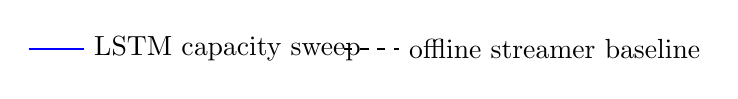
\begin{tikzpicture}[baseline=-0.5ex]
\draw[blue,thick] (0,0)--(0.7,0) node[right,black]{LSTM capacity sweep};
\draw[black,dashed,thick] (4.0,0)--(4.7,0) node[right,black]{offline streamer baseline};
\end{tikzpicture}
\end{center}

\begin{figure}[H]
\centering
\begin{minipage}{0.49\linewidth}\centering
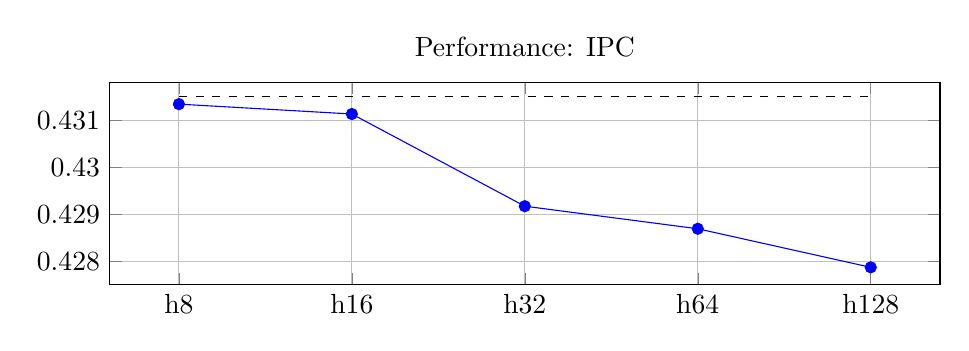
\begin{tikzpicture}\begin{axis}[
width=\linewidth,height=4.15cm,title={Performance: IPC},
xmode=log,log basis x=2,xtick={8,16,32,64,128},xticklabels={h8,h16,h32,h64,h128},
ymin=0.4275,ymax=0.4318,ytick={0.428,0.429,0.430,0.431},grid=major,
yticklabel style={/pgf/number format/fixed,/pgf/number format/precision=3}]
\addplot[blue,mark=*] coordinates {(8,0.43134)(16,0.43113)(32,0.42917)(64,0.42869)(128,0.42787)};
\addplot[black,dashed] coordinates {(8,0.43150)(128,0.43150)};
\end{axis}\end{tikzpicture}
\end{minipage}
\begin{minipage}{0.49\linewidth}\centering
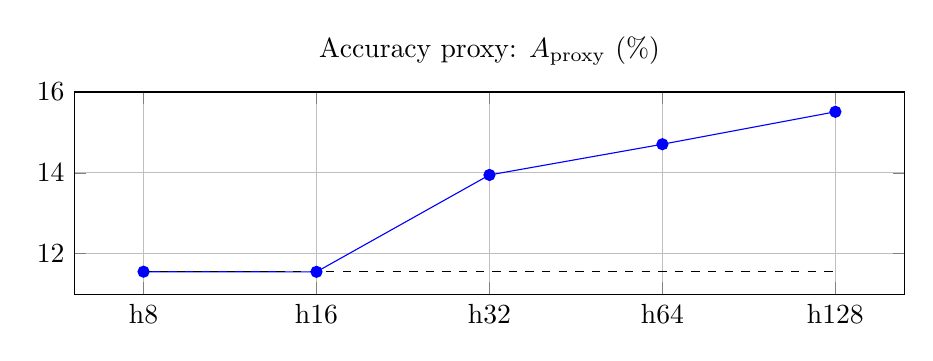
\begin{tikzpicture}\begin{axis}[
width=\linewidth,height=4.15cm,title={Accuracy proxy: $A_{\rm proxy}$ (\%)},
xmode=log,log basis x=2,xtick={8,16,32,64,128},xticklabels={h8,h16,h32,h64,h128},
ymin=11,ymax=16,grid=major]
\addplot[blue,mark=*] coordinates {(8,11.5558)(16,11.5527)(32,13.9475)(64,14.7075)(128,15.5093)};
\addplot[black,dashed] coordinates {(8,11.5622)(128,11.5622)};
\end{axis}\end{tikzpicture}
\end{minipage}

\begin{minipage}{0.49\linewidth}\centering
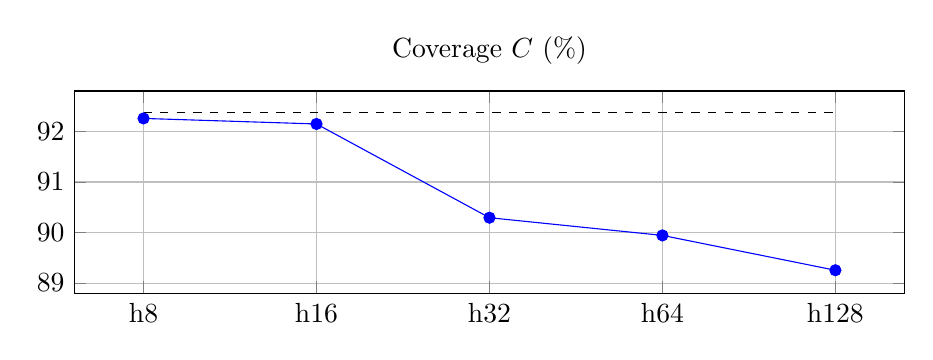
\begin{tikzpicture}\begin{axis}[
width=\linewidth,height=4.15cm,title={Coverage $C$ (\%)},
xmode=log,log basis x=2,xtick={8,16,32,64,128},xticklabels={h8,h16,h32,h64,h128},
ymin=88.8,ymax=92.8,grid=major]
\addplot[blue,mark=*] coordinates {(8,92.2567)(16,92.1469)(32,90.2930)(64,89.9429)(128,89.2537)};
\addplot[black,dashed] coordinates {(8,92.3744)(128,92.3744)};
\end{axis}\end{tikzpicture}
\end{minipage}
\begin{minipage}{0.49\linewidth}\centering
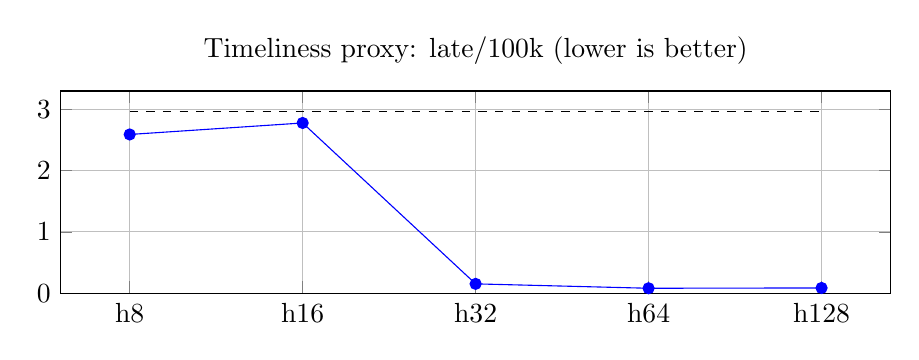
\begin{tikzpicture}\begin{axis}[
width=\linewidth,height=4.15cm,title={Timeliness proxy: late/100k (lower is better)},
xmode=log,log basis x=2,xtick={8,16,32,64,128},xticklabels={h8,h16,h32,h64,h128},
ymin=0,ymax=3.3,grid=major]
\addplot[blue,mark=*] coordinates {(8,2.5899)(16,2.7774)(32,0.1521)(64,0.0805)(128,0.0855)};
\addplot[black,dashed] coordinates {(8,2.9577)(128,2.9577)};
\end{axis}\end{tikzpicture}
\end{minipage}
\caption{The legend is outside the axes. Larger gates improve request-level yield and late density by suppressing traffic, but lose useful coverage and IPC.}
\end{figure}

\section*{Data-to-insight map}
\begin{center}\small
\begin{tabularx}{\textwidth}{@{}p{0.22\textwidth}p{0.32\textwidth}X@{}}
\toprule
Question & Data pattern & Supported insight \\
\midrule
Why does h8 miss the baseline? & $U:-239$, L2 misses:$+239$, late:$-6$. & Lost useful coverage dominates the tiny timeliness gain.\\
Why does apparent accuracy rise for h32--h128? & $A_{\rm proxy}$ rises to 13.95--15.51\%, while coverage falls to 90.29--89.25\%. & The ratio rises because requests are suppressed; this is not an end-to-end win.\\
Does more capacity help? & IPC decreases from h8 through h128; no crossing. & Capacity is not the bottleneck for this gate/objective.\\
\bottomrule
\end{tabularx}
\end{center}

\section*{Conclusion and evidence boundary}
\begin{itemize}
\item \textbf{Result:} no tested matched-input LSTM beats offline streamer; h8 is closest at $-0.00016$ IPC.
\item \textbf{Mechanism supported by current counters:} candidate suppression loses useful coverage faster than it improves late density.
\item \textbf{Not yet supported:} strict hardware accuracy, exact lead time, pollution, queue pressure, or cross-seed generalization.
\item \textbf{Next test:} keep the input/candidate contract fixed; optimize coverage-preserving utility and confirm a frozen design on a fresh window and additional seeds.
\end{itemize}

\section*{Verified provenance}
Analyzer status \texttt{PASS}; canonical content SHA256 prefixes: \texttt{2564c753145a} (train) and \texttt{36ce707c2f27} (evaluation). Live streamer is a validated reference (0.43161 IPC), not the primary offline comparator.

\end{document}
